\documentclass[12pt]{extarticle}

\usepackage{amsmath}
\usepackage{unicode-math}
\usepackage{xltxtra}
\usepackage{xgreek}

\setmainfont{Liberation Serif}

\usepackage{tabularx}

\pagestyle{empty}

\usepackage{geometry}
\geometry{a4paper, total={190mm,275mm}, left=10mm, top=10mm}

\usepackage{graphicx}
\graphicspath{ {images/} }

\usepackage{wrapfig}

\begin{document}
\renewcommand{\labelenumi}{\alph{enumi})}
\renewcommand{\labelenumii}{\roman{enumii}.}

\section*{Θέμα 1}
\noindent

\begin{enumerate}
    \item Να αποδείξετε ότι το εμβαδόν Ε ενός τριγώνου είναι ίσο με το ημιγινόμενο μιας πλευράς επί το αντίστοιχο ύψος. \hspace*{\fill} \textbf{Μονάδες 15}

          Απόδειξη από βιβλίο
    \item Να χαρακτηρίσετε τις παρακάτω προτάσεις με Σωστό ή Λάθος
          \begin{enumerate}
              \item Λ Το τετράγωνο της κάθετης πλευράς ενός ορθογωνίου τριγώνου ισούται με το γινόμενο της κάθετης πλευράς με την υποτείνουσα.
              \item Σ Το μήκος ενός τόξου $α$ ακτινίων σε κύκλο ακτίνας $R$ είναι $l=αR$.
              \item Λ Ο λόγος ομοιότητας των εμβαδών δύο όμοιων σχημάτων ισούται με τον λόγο ομοιότητας των πλευρών του.
              \item Λ Κανονικό πολύγωνο είναι το σχήμα που έχει όλες τις πλευρές του ίσες.
              \item Σ Σε τρίγωνο με πλευρές $α$, $β$, $γ$, αν ισχύει $β^2<α^2+γ^2$ τότε $\hat{Β}<90^{\circ}$.\hspace*{\fill}\textbf{Μονάδες 10}
          \end{enumerate}
\end{enumerate}

\section*{Θέμα 2 (21350)}
\noindent
Στο σχήμα δίνονται ότι $\hat{Β}=\hat{Ε}=90^{\circ}$, $ΑΕ=8$, $ΕΒ=4$ και $ΔΕ=4$.
\begin{enumerate}
    \item[α)] Να αποδείξετε ότι τα τρίγωνα $ΑΕΔ$ και $ΑΒΓ$ είναι όμοια \hspace*{\fill} \textbf{Μονάδες 10}

        Αρκεί να δείξουμε ότι έχουν 2 ίσες γωνίες. Είναι ορθογώνια τρίγωνα και έχουν μία οξεία γωνία ίση.

    \item[β)] Να γράψετε τους ίσους λόγους που προκύπτουν από την ομοιότητα των τριγώνων $ΑΕΔ$ και $ΑΒΓ$

        \hspace*{\fill} \textbf{Μονάδες 10}

        $$\dfrac{ΑΕ}{ΑΒ}=\dfrac{ΑΔ}{ΑΓ}=\dfrac{ΔΕ}{ΒΓ}$$
    \item[γ)] Να υπολογίσετε το μήκος της πλευράς $ΒΓ$ \hspace*{\fill} \textbf{Μονάδες 5}

        Από πριν $\dfrac{ΑΕ}{ΑΒ}=\dfrac{ΔΕ}{ΒΓ}\implies ΒΓ=6$
\end{enumerate}
\begin{figure}[h]

    \centering
    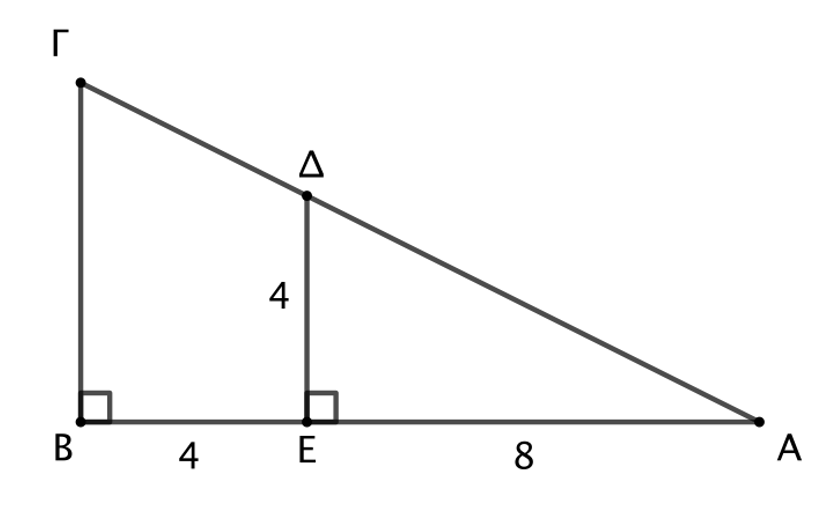
\includegraphics[width=0.50\textwidth]{2023(2)}
\end{figure}

\section*{Θέμα 3}
\noindent

\begin{wrapfigure}[3]{r}{0.38\textwidth}
    \centering
    \vspace{-20pt}
    \hspace{-80pt}
    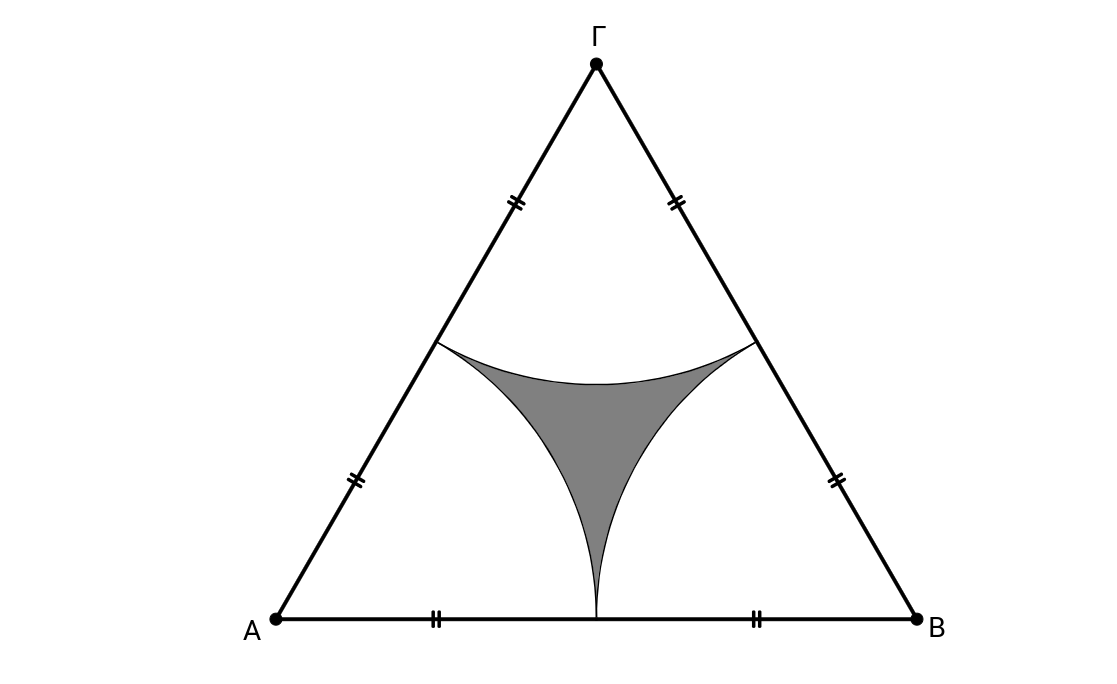
\includegraphics[width=0.38\textwidth]{2017BGeo3}
\end{wrapfigure}

Έστω ισόπλευρο τρίγωνο πλευράς $2R$. Με κέντρο κάθε κορυφή εγγράφουμε στο τρίγωνο κυκλικούς τομείς ακτίνας $R$ όπως το διπλανό σχήμα.
\begin{enumerate}
    \item[α)] Να βρείτε την περίμετρο του γραμμοσκιασμένου σχήματος ως προς $R$. \hspace*{\fill} \textbf{Μονάδες 9}

        Οι γωνίες του τριγώνου είναι όλες $60^ο$, άρα οι 3 κυκλικοί τομείς σχηματίζουν ημικύκλιο. Άρα η περίμετρος είναι $\dfrac{2πR}{2}=πR$
    \item[β)] Να δείξετε ότι το ύψος του τριγώνου είναι $R\sqrt{3}$. \hspace*{\fill} \textbf{Μονάδες 4}

        Με Π.Θ. έχουμε $(2R)^2=R^2+υ^2\implies ...$
    \item[γ)] Να δείξετε ότι το εμβαδό του τριγώνου είναι $R^2\sqrt{3}$. \hspace*{\fill} \textbf{Μονάδες 3}

        Το εμβαδό του τριγώνου είναι $\dfrac{2}{2}2R\cdot υ=...$
    \item[δ)] Να υπολογίσετε το εμβαδό του γραμμοσκιασμένου τμήματος ως προς $R$. \hspace*{\fill} \textbf{Μονάδες 9}

        Από το εμβαδό του τριγώνου αφαιρούμε το ημικύκλιο που αναφερόμαστε στο α). Άρα $R^2\sqrt{3}-\dfrac{πR^2}{2}$
\end{enumerate}

\section*{Θέμα 4 (16135)}
\noindent

Δίνεται το τρίγωνο $ΑΒΓ$ με υποτείνουσα $ΒΓ=10$ και έστω ότι $Δ$ είναι η προβολή της κορυφής $Α$ στην $ΒΓ$.
\begin{enumerate}
    \item[α)] Αν $ΔΒ=2$ να υπολογίσετε
        \begin{enumerate}
            \item το ύψος $ΑΔ$ του τριγώνου $ΑΒΓ$ \hspace*{\fill} \textbf{Μονάδες 7}

                  Ισχύει $ΑΔ^2=ΒΔ\cdot ΔΓ \implies ΑΔ=4$
            \item το εμβαδόν του τριγώνου $ΑΒΓ$ \hspace*{\fill} \textbf{Μονάδες 5}

                  $Ε=\dfrac{1}{2}ΒΓ\cdot ΑΔ = 5ΑΔ = 20$
        \end{enumerate}

    \item[β)] Υποθέστε ότι το σημείο $Α$ κινείται πάνω στο ημικύκλιο με διάμετρο την $ΒΓ$
        \begin{enumerate}
            \item Να ποδείξετε ότι το εμβαδόν του τριγώνου $ΑΒΓ$ είναι $(ΑΒΓ)=5ΑΔ$ \hspace*{\fill} \textbf{Μονάδες 7}

                  Αποδείχθηκε πιο πάνω
            \item Θεωρήστε τον παρακάτω ισχυρισμό:

                  "Για όλες τις θέσεις του $Α$ πάνω στο ημικύκλιο με διάμετρο την $ΒΓ$, το εμβαδόν του τριγώνου $ΑΒΓ$ δεν υπερβαίνει το 25"

                  Είναι αληθής ή ψευδής ο παραπάνω ισχυρισμός; Να αιτιολογήσετε την απάντησή σας. \hspace*{\fill} \textbf{Μονάδες 6}


                  Αληθής. Με σταθερή βάση, το τρίγωνο έχει μέγιστο εμβαδό, στο μέγιστο ύψος. Το ύψος δεν μπορεί να ξεπερνάει την ακτίνα του κύκλου, δηλαδή $υ=ΑΔ \le 5$. Έτσι $Ε\le 25$
        \end{enumerate}
\end{enumerate}
\begin{figure}[h]

    \centering
    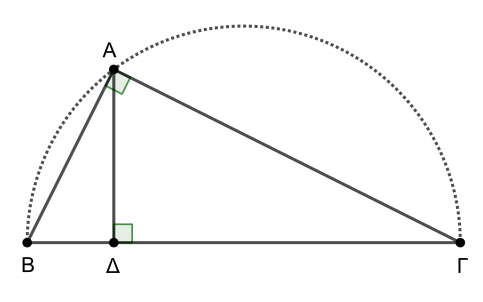
\includegraphics[width=0.50\textwidth]{2023(4)}
\end{figure}
\end{document}